\section{eo\-Normal\-Init$<$ T $>$ Class Template Reference}
\label{classeo_normal_init}\index{eoNormalInit@{eoNormalInit}}
The class {\bf normal\_\-generator}{\rm (p.\,\pageref{classnormal__generator})} can be used in the STL generate function to easily generate gaussian distributed floats and doubles.  


{\tt \#include $<$eo\-Uniform\-Init.h$>$}

Inheritance diagram for eo\-Normal\-Init$<$ T $>$::\begin{figure}[H]
\begin{center}
\leavevmode
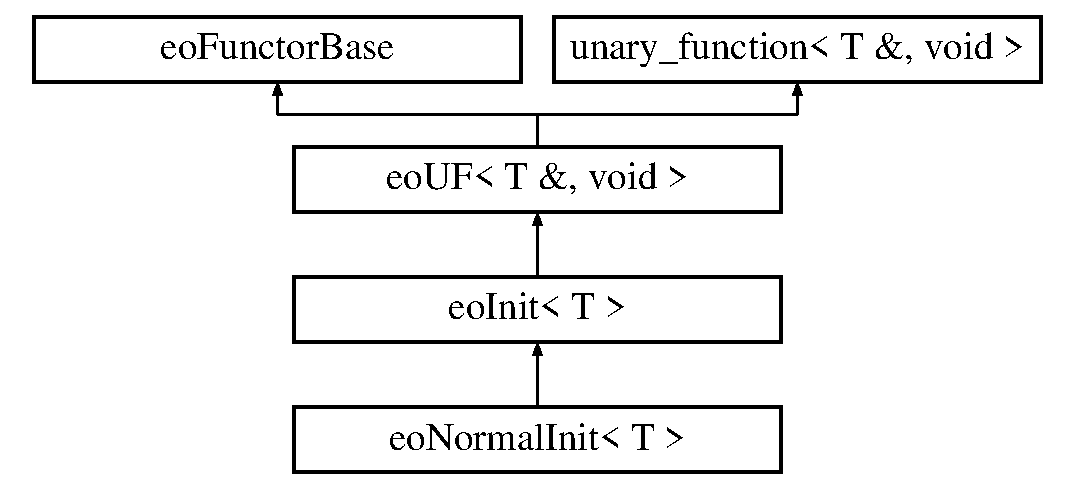
\includegraphics[height=4cm]{classeo_normal_init}
\end{center}
\end{figure}
\subsection*{Public Member Functions}
\begin{CompactItemize}
\item 
{\bf eo\-Normal\-Init} (T \_\-stdev=T(1.0), {\bf eo\-Rng} \&\_\-rng=rng)\label{classeo_normal_init_a0}

\item 
void {\bf operator()} (T \&\_\-t)\label{classeo_normal_init_a1}

\begin{CompactList}\small\item\em The pure virtual function that needs to be implemented by the subclass. \item\end{CompactList}\end{CompactItemize}
\subsection*{Private Attributes}
\begin{CompactItemize}
\item 
T {\bf stdev}\label{classeo_normal_init_r0}

\item 
{\bf eo\-Rng} \& {\bf normal}\label{classeo_normal_init_r1}

\end{CompactItemize}


\subsection{Detailed Description}
\subsubsection*{template$<$class T = double$>$ class eo\-Normal\-Init$<$ T $>$}

The class {\bf normal\_\-generator}{\rm (p.\,\pageref{classnormal__generator})} can be used in the STL generate function to easily generate gaussian distributed floats and doubles. 

The user can supply a standard deviation which defaults to 1. 



Definition at line 126 of file eo\-Uniform\-Init.h.

The documentation for this class was generated from the following file:\begin{CompactItemize}
\item 
eo\-Uniform\-Init.h\end{CompactItemize}
